\section{Partial Derivatives}

\subsection{Definition and Properties of Partial Derivatives}
\begin{definition}{Partial Derivative}{partial_derivative}
    In this course, we will focus on functions of two variables, i.e., $f(x, y)$.
    For a binary function $f(x, y)$, the partial derivative with respect to $x$ is given by:
    \[
        \pdv{f}{x} = \lim_{h \to 0} \frac{f(x + h, y) - f(x, y)}{h}
    \]
    and the partial derivative with respect to $y$ is given by:
    \[
        \pdv{f}{y} = \lim_{h \to 0} \frac{f(x, y + h) - f(x, y)}{h}
    \]
    provided these limits exist.
    
    In general, let $f(x_1, x_2, \ldots, x_n)$ be a function of $n$ variables. The \textbf{partial derivative} of $f$ with respect to the variable $x_i$ is defined as:
    \[
        \pdv{f}{x_i} = \lim_{h \to 0} \frac{f(x_1, x_2, \ldots, x_i + h, \ldots, x_n) - f(x_1, x_2, \ldots, x_i, \ldots, x_n)}{h}
    \]
    provided this limit exists.
\end{definition}

Some key points to note about partial derivatives:
\begin{itemize}
    \item $f_x(a, b)$ is the instantaneous rate of change of $f$ at the point $(a, b)$ in the $x$-direction.
    \item $f_x(a, b)$ is the slope of the tangent line to $f(a, b)$ at the point $x = a$.
\end{itemize}

Computing partial derivatives is similar to computing derivatives in single-variable calculus.
The only difference is that we treat all other variables as constants when differentiating with respect to one variable.

\begin{example}[Partial Derivatives of a Binary Function]
Let $f(x, y) = e^{2x} \cos(y)$.

We can now compute the partial derivatives of $f$ with respect to $x$ and $y$:
\begin{align*}
    f_x(x, y) &= \pdv{}{x} \left( e^{2x} \cos(y) \right) = 2 e^{2x} \cos(y) \\
    f_y(x, y) &= \pdv{}{y} \left( e^{2x} \cos(y) \right) = -e^{2x} \sin(y)
\end{align*}
\end{example}

For better comprehension, we can visualize the partial derivatives of a function of two variables as the slopes of tangent lines to the surface defined by the function in the $x$ and $y$ directions.

\begin{example}[Visualizing Partial Derivatives]

Consider the surface defined by
$f(x, y) = -\frac{10y}{e^{x^2 + y^2}}$
and its slices along fixed coordinate planes.

\vspace{0.5em}

% --- Row 1: Original Surface ---
\noindent
\begin{minipage}[c]{0.52\textwidth}
\centering
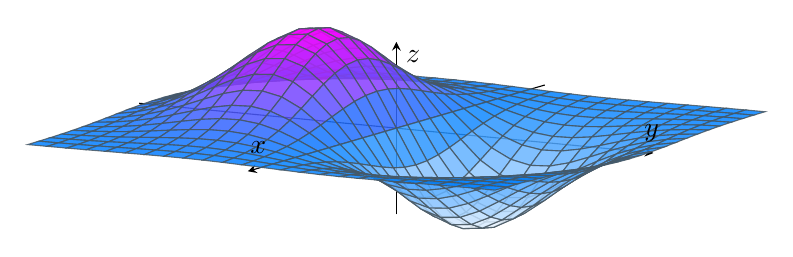
\begin{tikzpicture}
\begin{axis}[
    view={120}{30},
    axis lines=center,
    xlabel={$x$}, ylabel={$y$}, zlabel={$z$},
    xmin=-2.2, xmax=2.2,
    ymin=-2.2, ymax=2.2,
    zmin=-4, zmax=4,
    ticks=none,
    width=0.98\textwidth,
    height=5.5cm
]
    \addplot3[
        surf,
        domain=-2:2,
        domain y=-2:2,
        samples=25,
        colormap/cool,
        faceted color=cyan!30!black,
        thin,
        opacity=0.85
    ] {-10*y*exp(-x^2-y^2)};
\end{axis}
\end{tikzpicture}
\end{minipage}%
\begin{minipage}[c]{0.46\textwidth}
\centering
\textit{(Original surface $z=f(x,y)$)}
\end{minipage}

\vspace{1em}

% --- Row 2: x = 1 Trace ---
\noindent
\begin{minipage}[c]{0.52\textwidth}
\centering
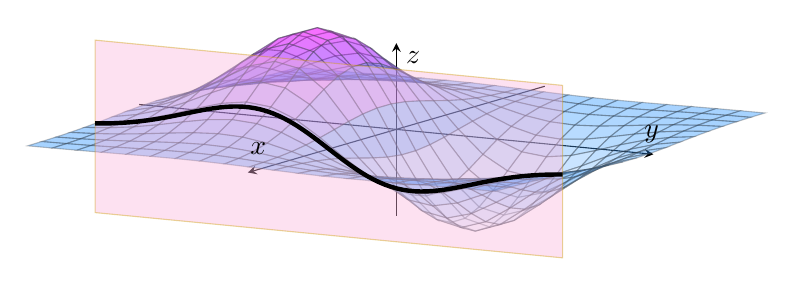
\begin{tikzpicture}
\begin{axis}[
    view={120}{30},
    axis lines=center,
    xlabel={$x$}, ylabel={$y$}, zlabel={$z$},
    xmin=-2.2, xmax=2.2,
    ymin=-2.2, ymax=2.2,
    zmin=-4, zmax=4,
    ticks=none,
    clip=false,
    width=0.98\textwidth,
    height=5.5cm
]
    % Surface
    \addplot3[
        surf,
        domain=-2:2,
        domain y=-2:2,
        samples=20,
        colormap/cool,
        opacity=0.35,
        faceted color=cyan!20!black
    ] {-10*y*exp(-x^2-y^2)};

    % Plane x = 1
    \addplot3[
        surf,
        domain=-2:2,
        domain y=-4:4,
        samples=2,
        samples y=2,
        color=magenta!30,
        opacity=0.4
    ] (1,x,y);

    % Trace curve at x = 1
    \addplot3[
        domain=-2:2,
        samples=80,
        samples y=0,
        variable=\t,
        color=black,
        ultra thick
    ] (1,\t,{-10*\t*exp(-1-\t^2)});
\end{axis}
\end{tikzpicture}
\end{minipage}%
\begin{minipage}[c]{0.46\textwidth}

\textbf{$x=1$ Trace:}

\[
z=f(1,y)=-\frac{10y}{e^{1+y^2}}
\]

\centering
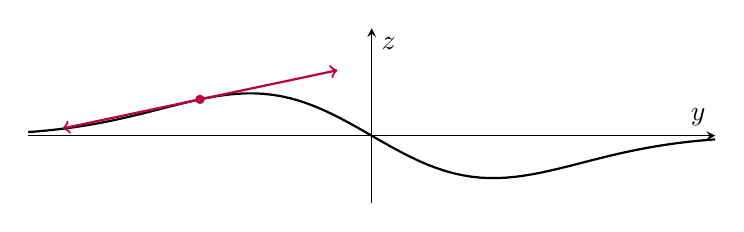
\begin{tikzpicture}
\begin{axis}[
    axis lines=center,
    xlabel={$y$}, ylabel={$z$},
    xmin=-2, xmax=2,
    ymin=-2.5, ymax=4,
    ticks=none,
    width=0.85\textwidth,
    height=3.8cm
]
    \addplot[
        domain=-2:2,
        samples=80,
        thick,
        color=black
    ] {-10*x*exp(-1-x^2)};

    % Tangent line at y = -1
    \addplot[
        domain=-1.8:-0.2,
        color=purple,
        thick,
        <->
    ] {10/exp(2)*(x+2)};

    \node[
        circle,
        fill=purple,
        inner sep=1.2pt
    ] at (axis cs:-1,{10/exp(2)}) {};
\end{axis}
\end{tikzpicture}

\raggedright

At $(1,-1)$,
\[
f_y(1,-1)=\frac{10}{e^2}>0.
\]

\end{minipage}

\vspace{1em}

% --- Row 3: y = -1 Trace ---
\noindent
\begin{minipage}[c]{0.52\textwidth}
\centering
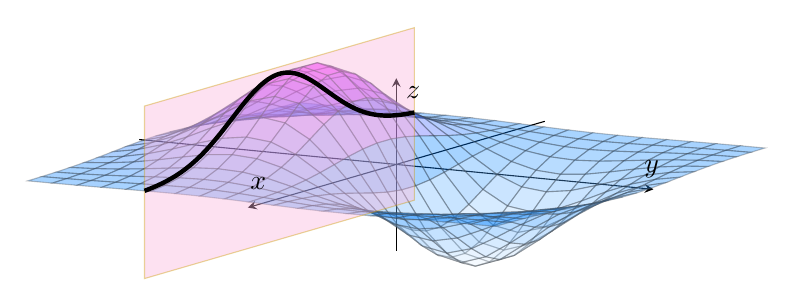
\begin{tikzpicture}
\begin{axis}[
    view={120}{30},
    axis lines=center,
    xlabel={$x$}, ylabel={$y$}, zlabel={$z$},
    xmin=-2.2, xmax=2.2,
    ymin=-2.2, ymax=2.2,
    zmin=-4, zmax=4,
    ticks=none,
    clip=false,
    width=0.98\textwidth,
    height=5.5cm
]
    % Surface
    \addplot3[
        surf,
        domain=-2:2,
        domain y=-2:2,
        samples=20,
        colormap/cool,
        opacity=0.35,
        faceted color=cyan!20!black
    ] {-10*y*exp(-x^2-y^2)};

    % Plane y = -1
    \addplot3[
        surf,
        domain=-2:2,
        domain y=-4:4,
        samples=2,
        samples y=2,
        color=magenta!30,
        opacity=0.4
    ] (x,-1,y);

    % Trace curve at y = -1
    \addplot3[
        domain=-2:2,
        samples=80,
        samples y=0,
        variable=\t,
        color=black,
        ultra thick
    ] (\t,-1,{10*exp(-\t^2-1)});
\end{axis}
\end{tikzpicture}
\end{minipage}%
\begin{minipage}[c]{0.46\textwidth}

\textbf{$y=-1$ Trace:}

\[
z=f(x,-1)=\frac{10}{e^{x^2+1}}
\]

\centering
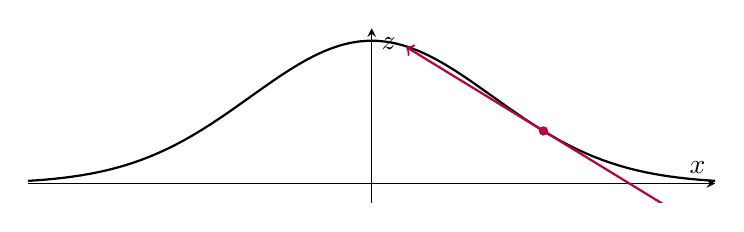
\begin{tikzpicture}
\begin{axis}[
    axis lines=center,
    xlabel={$x$}, ylabel={$z$},
    xmin=-2, xmax=2,
    ymin=-0.5, ymax=4,
    ticks=none,
    width=0.85\textwidth,
    height=3.8cm
]
    \addplot[
        domain=-2:2,
        samples=80,
        thick,
        color=black
    ] {10*exp(-x^2-1)};

    % Tangent line at x = 1
    \addplot[
        domain=0.2:1.8,
        color=purple,
        thick,
        <->
    ] {10/exp(2)-20/exp(2)*(x-1)};

    \node[
        circle,
        fill=purple,
        inner sep=1.2pt
    ] at (axis cs:1,{10/exp(2)}) {};
\end{axis}
\end{tikzpicture}

\raggedright

At $(1,-1)$,
\[
f_x(1,-1)=-\frac{20}{e^2}<0.
\]

\end{minipage}

\end{example}

\vspace{1.5em}

% --- Problem Section: Contour Map Analysis ---
\begin{problem}{Visualizing Partial Derivatives on a Contour Map}{}
Give some reasonable labelings to the contour map based on the image of the graph above.

\vspace{0.5em}
\begin{center}
\begin{tikzpicture}
\begin{axis}[
    view={0}{90},
    grid=both,
    grid style={line width=.1pt, draw=gray!30},
    major grid style={line width=.2pt, draw=gray!60},
    axis lines=middle,
    xlabel={$x$},
    ylabel={$y$},
    xmin=-2.2, xmax=2.2,
    ymin=-1.8, ymax=1.8,
    xtick={-2,-1.5,-1,-0.5,0,0.5,1,1.5,2},
    ytick={-1.5,-1,-0.5,0,0.5,1,1.5},
    width=0.85\textwidth,
    height=7.5cm,
    enlargelimits=false,
]

% --- Contour map ---
\addplot3[
    contour gnuplot={
        levels={
            -5.0,
            -3.8,
            -2.2,
            -1.35335,
            1.35335,
            2.2,
            3.8,
            5.0
        },
        labels=false,
        draw color=red!80!black,
        contour label style={
            /pgf/number format/fixed,
            /pgf/number format/precision=2
        }
    },
    domain=-2.2:2.2,
    domain y=-1.8:1.8,
    samples=100,
    thick
]
{-10*y*exp(-x^2-y^2)};

% --- Points O, P, R ---
\addplot[
    only marks,
    mark=*,
    mark size=2.2pt,
]
coordinates {
    (1,1)
    (1,-1)
};

% --- Labels ---
\node[above right] at (axis cs:1,1) {$P(1,1)$};
\node[below right] at (axis cs:1,-1) {$R(1,-1)$};

\end{axis}
\end{tikzpicture}
\end{center}

\vspace{0.5em}
Determine whether the following values are \textbf{positive}, \textbf{negative}, or \textbf{0}:
\begin{enumerate}
    \item $f_x(O)$ and $f_y(O)$ at the origin $O(0,0)$.
    \item $f_x(P)$ and $f_y(P)$ at $P(1, 1)$.
    \item Compare $|f_x(R)|$ and $|f_y(R)|$ at $R(1, -1)$. Which is greater?
\end{enumerate}
\end{problem}

\begin{sol}
\begin{enumerate}
    \item At $O(0,0)$:
    \[ f_x(0,0) = 0 , f_y(0,0) = -10 < 0 \]
    
    \item At $P(1,1)$:
    As $x$ increases, $f(x,1)$ increases towards $0$ from negative values, so $f_x(P) > 0$.
    At $y = 1$, $f(1,y)$ reaches a local extremum, so $f_y(P) = 0$.
    
    \item At $R(1,-1)$:
    The contour lines are significantly denser in the $y$-direction than in the $x$-direction. Thus:
    \[ |f_x(R)| > |f_y(R)| \]
\end{enumerate}
\end{sol}

\subsection{Linear Approximation}

\begin{definition}{Linear Function}{linear_function}
A \textbf{linear function} of two variables is a function of the form
\[
    f(x, y) = m_x x + m_y y + c
\]
\end{definition}

The idea of linear approximation is to approximate a function $f(x, y)$ by a linear function $L(x, y)$ that is tangent to the surface defined by $f$ at a given point $(a, b)$.

Given a function $L(x, y) = m_x (x - a) + m_y (y - b) + C$.

Firstly, we want $L(a, b) = f(a, b)$.
We then write the linear function as
\[
    L(x, y) = m_x (x - a) + m_y (y - b) + f(a, b)
\]

Secondly, we want the traces of $L$ to be tangent to the traces of $f$ at $(a, b)$.
Hence, we have
\[
    m_x = f_x(a, b), \quad m_y = f_y(a, b)
\]
Therefore,
\[
    L(x, y) = f_x(a, b)\cdot(x - a) + f_y(a, b)\cdot(y - b) + f(a, b)
\]

Thus, we now have the following definition of linear approximation:
\begin{definition}{Linear Approximation}{linear_approximation}
The \textbf{linear approximation} of a function $f(x, y)$ at the point $(a, b)$ is given by
\[
    z = f(a, b) + f_x(a, b)(x - a) + f_y(a, b)(y - b),
\]
which is the tangent plane.
\end{definition}

\begin{problem}{Finding a Linear Approximation}{linear_approximation_problem}
Find the linear approximation of $f(x, y) = \frac{x^2}{y^2+1}$ at $(4, 1)$. 
Use your answer to approximate $f(4.01, 0.98)$.
\end{problem}

\begin{sol}
First, we find the partial derivatives of $f(x, y) = \frac{x^2}{y^2+1}$:
\[
    f_x(x, y) = \frac{2x}{y^2+1}, \quad f_y(x, y) = -\frac{2x^2y}{(y^2+1)^2}
\]
At the point $(4, 1)$:
\[
    f(4, 1) = \frac{16}{2} = 8, \quad f_x(4, 1) = \frac{8}{2} = 4, \quad f_y(4, 1) = -\frac{32}{4} = -8
\]
The linear approximation is:
\[
    z = 8 + 4(x - 4) + (-8)(y - 1)
\]
Simplifying:
\[
    z = 8 + 4x - 16 - 8y + 8 = 4x - 8y
\]
To approximate $f(4.01, 0.98)$:
\[
    f(4.01, 0.98) \approx 4(4.01) - 8(0.98) = 16.04 - 7.84 = 8.2
\]
\end{sol}

\subsection{Differentiability}

\begin{definition}{Differentiability}{differentiability}
A function $f(x, y)$ is said to be \textbf{differentiable} at a point $(a, b)$ if the linear approximation of $f$ at $(a, b)$ is a good approximation of $f$ near $(a, b)$.

This is equivalent to saying that $f(x, y)$ has a tangent plane at $(a, b)$.

A formal definition of differentiability is as follows:
\[
    \lim_{(x, y) \to (a, b)} \dfrac{f(x, y) - L(x, y)}{\sqrt{(x - a)^2 + (y - b)^2}} = 0
\]
\end{definition}

\begin{example}[\textbf{Non-example:}]
\[
    g(x, y) = \begin{cases} \dfrac{2xy(x+y)}{x^2+y^2} & (x,y) \neq (0,0) \\[10pt] 0 & (x,y) = (0,0) \end{cases}.
\]
\begin{center}
    % Polar parametrization for g(x,y) to handle the discontinuity seamlessly at (0,0):
% g(r, theta) = r * sin(2*theta) * (cos(theta) + sin(theta))
\def\funcG(#1,#2){ (#1 * sin(2*#2) * (cos(#2) + sin(#2))) }

\begin{tikzpicture}
\begin{axis}[
    view={120}{30},
    axis lines=center,
    xlabel={$x$}, ylabel={$y$}, zlabel={$z$},
    xmin=-1.6, xmax=1.6,
    ymin=-1.6, ymax=1.6,
    zmin=-1.6, zmax=1.6,
    ticks=none,
    clip=false,
    width=0.8\textwidth,
    height=7.5cm,
    z buffer=sort
]
    % Main surface: g(x,y) using polar parametrization
    \addplot3[
        surf,
        colormap/cool,
        opacity=0.35,
        faceted color=cyan!20!black,
        domain=0:1.5,         % radius r
        domain y=0:360,       % angle theta in degrees
        samples=15,
        samples y=72,
        shader=faceted
    ] (
        {x*cos(y)},
        {x*sin(y)},
        {\funcG(x,y)}
    );

    % Highlight point at the origin (0,0,0) where partial derivatives exist
    \node[
        circle, fill=red!60, inner sep=1.2pt,
        label={[text=red!60]below left:$(0,0)$}
    ] at (axis cs:0,0,0) {};
\end{axis}
\end{tikzpicture}
\end{center}

Note that in single variable calculus, if a function has a derivative at a point, it is also differentiable at that point.
However, in multivariable calculus, this is not necessarily the case.

This function $g(x, y)$ is a tricky function.
From calculation, we know its partial derivatives, $\displaystyle\pdv{g}{x}$ and $\displaystyle\pdv{g}{y}$, exist at $(0, 0)$:
\begin{align*}
    g_x(0, 0) &= \lim_{h \to 0} \frac{g(h, 0) - g(0, 0)}{h} \\ 
              &= \lim_{h \to 0} \frac{0 - 0}{h} = 0 \\
    g_y(0, 0) &= \lim_{h \to 0} \frac{g(0, h) - g(0, 0)}{h} \\
              &= \lim_{h \to 0} \frac{0 - 0}{h} = 0
\end{align*}

In fact, from all directions, the derivatives of $g$ exists.

However, $g$ is not \textbf{differentiable} at $(0, 0)$.

To show this, we can use the definition of differentiability.
\begin{align*}
    \lim_{(x, y) \to (0, 0)} \dfrac{g(x, y) - L(x, y)}{\sqrt{x^2 + y^2}} &= \lim_{(x, y) \to (0, 0)} \dfrac{g(x, y) - g(0, 0) + g_x(0, 0)(x - 0) + g_y(0, 0)(y - 0)}{\sqrt{x^2 + y^2}} \\[0.5em]
    &= \lim_{(x, y) \to (0, 0)} \dfrac{g(x, y)}{\sqrt{x^2 + y^2}} \\[0.5em]
    &= \lim_{(x, y) \to (0, 0)} \dfrac{2xy(x+y)}{(x^2+y^2)\sqrt{x^2 + y^2}} \\[0.5em]
    &= \lim_{(x, y) \to (0, 0)} \dfrac{2xy(x+y)}{(x^2+y^2)^{3/2}}
\end{align*}

We approach $(0, 0)$ along the line $y = x$:
\begin{align*}
    \lim_{(x, y) \to (0, 0)} \dfrac{2xy(x+y)}{(x^2+y^2)^{3/2}} &= \lim_{x \to 0} \dfrac{2x \cdot x(x+x)}{(x^2+x^2)^{3/2}} \\[0.5em]
    &= \lim_{x \to 0} \dfrac{2x^2(2x)}{(2x^2)^{3/2}} \\[0.5em]
    &= \lim_{x \to 0} \dfrac{4x^3}{(2x^2)^{3/2}} \\[0.5em]
    &= \lim_{x \to 0} \dfrac{4x^3}{2^{3/2} x^3} \\[0.5em]
    &= \lim_{x \to 0} \dfrac{4}{2^{3/2}} \\[0.5em]
    &= \dfrac{4}{2\sqrt{2}} = \sqrt{2} \neq 0
\end{align*}

This shows that linear approximation is not a good approximation of $g$ near $(0, 0)$, and hence $g$ is not differentiable at $(0, 0)$.

We now introduce a theorem that provides a sufficient condition for differentiability.
\begin{theorem}{Sufficient Condition for Differentiability}{sufficient_condition_for_differentiability}
    If $f_x$ and $f_y$ are continuous on an open disk $D$, then $f(x, y)$ is differentiable on $D$.
\end{theorem}

\end{example}

\subsection{Higher-Order Partial Derivatives}

\begin{definition}{Higher-Order Partial Derivatives}{higher_order_partial_derivatives}
We denote by $f_{xx}$ the function
\[
    f_{xx}(x, y) = \pdv{}{x} \left( \pdv{f}{x} \right) = \pdv{f}{x}
\]
and similarly for $f_{yy}$.

We denote by $f_{xy}$ the function
\[
    f_{xy}(x, y) = \pdv{}{y} \left( \pdv{f}{x} \right) = \pdv{f}{x}{y}
\]
and similarly for $f_{yx}$.

\textbf{Note that the order of differentiation matters for mixed partial derivatives.}
\end{definition}

The interpretation of higher-order partial derivatives is similar to that of first-order partial derivatives.
\begin{itemize}
    \item $f_{xx}(a, b)$ is the instantaneous rate of change of $f_x$ at the point $(a, b)$ in the $x$-direction.
    \item $f_{xy}(a, b)$ is the instantaneous rate of change of $f_x$ at the point $(a, b)$ in the $y$-direction.
    \item $f_{yx}(a, b)$ is the instantaneous rate of change of $f_y$ at the point $(a, b)$ in the $x$-direction.
\end{itemize}

\begin{theorem}{Clairaut's Theorem}{clairauts_theorem}
    Suppose that $f_{xy}$ and $f_{yx}$ are continuous on some open disk $D$. Then
    \[
        f_{xy}(a, b) = f_{yx}(a, b) \quad \text{for all } (a, b) \in D
    \]
    It is similar for functions of more than two variables.
\end{theorem}

\begin{example}[Application of Clairaut's Theorem]
Let $g(x, y, z, w) = x^3w^2z^2+ \sin\left(\dfrac{xy}{z^2}\right)$.
Now we want to find $g_{zzwx}$.

First, we examine the function $g$.
Notice that the first term, $x^3w^2z^2$, is a polynomial function, which is infinitely differentiable over $\mathbb{R}^n$.

The second term, $\sin\left(\dfrac{xy}{z^2}\right)$, is a composite function. However, $\sin$ is infinitely differentiable over $\mathbb{R}$, and $\dfrac{xy}{z^2}$ also infinitely differentiable over $\mathbb{R}^n, z \neq 0$.

Hence, $g$ is infinitely differentiable over $\mathbb{R}^n, z \neq 0$.

This gives that 
\[
g_{zzwx} = \pdv{g}{z,z,w,x} = g_{wzzx} = g_{xwzz} = \cdots
\]

If we calculate this in the original order, we have
\begin{align*}
    g_{zzwx} &= (((g_z)_z)_w)_x \\
    &= (((6x^3w^2z - \frac{2y}{z^3}\cos\left(\dfrac{xy}{z^2}\right) - \frac{2xy^2}{z^5}\sin\left(\dfrac{xy}{z^2}\right))_z)_w)_x \\
    &= (((6x^3w^2 + \frac{6y}{z^4}\cos\left(\dfrac{xy}{z^2}\right) + \frac{10xy^2}{z^6}\sin\left(\dfrac{xy}{z^2}\right) - \frac{4x^2y^3}{z^8}\cos\left(\dfrac{xy}{z^2}\right))_w)_x \\
    &= \cdots
\end{align*}

We want to try to avoid this tedious calculation by using Clairaut's Theorem.
Rearranging the order of differentiation to $g_{xwzz}$, we have
\begin{align*}
    g_{xwzz} &= (((g_x)_w)_z)_z \\
    &= (((3x^2w^2z^2 + \frac{y}{z^2}\cos\left(\dfrac{xy}{z^2}\right))_w)_z)_z \\
    &= (((6x^2wz^2 + 0)_z)_z) \\
    &= ((12x^2wz + 0)_z) \\
    &= 12x^2w
\end{align*}
\end{example}

